\section{Analysis}
This section presents detailed analysis on the benefits of effective localization on issue resolution (\S\ref{sec:downstream_swebench}) and the evolving tool-use behaviors during RL (\S\ref{sec:tool_use_behaviour}). Appendix \ref{appendix:error_analysis} includes detailed error analysis of \methodname models.

\subsection{Does Effective Code Localization Improve Issue Resolution?}\label{sec:downstream_swebench}
\begin{figure*}[!t]
    \centering
    % Define specific dimensions to ensure uniformity
    \newcommand{\figwidth}{0.49\textwidth}
    \newcommand{\figheight}{4.5cm} % Adjust this value until the aspect ratio looks natural
        \begin{subfigure}[b]{\figwidth}
        \centering
        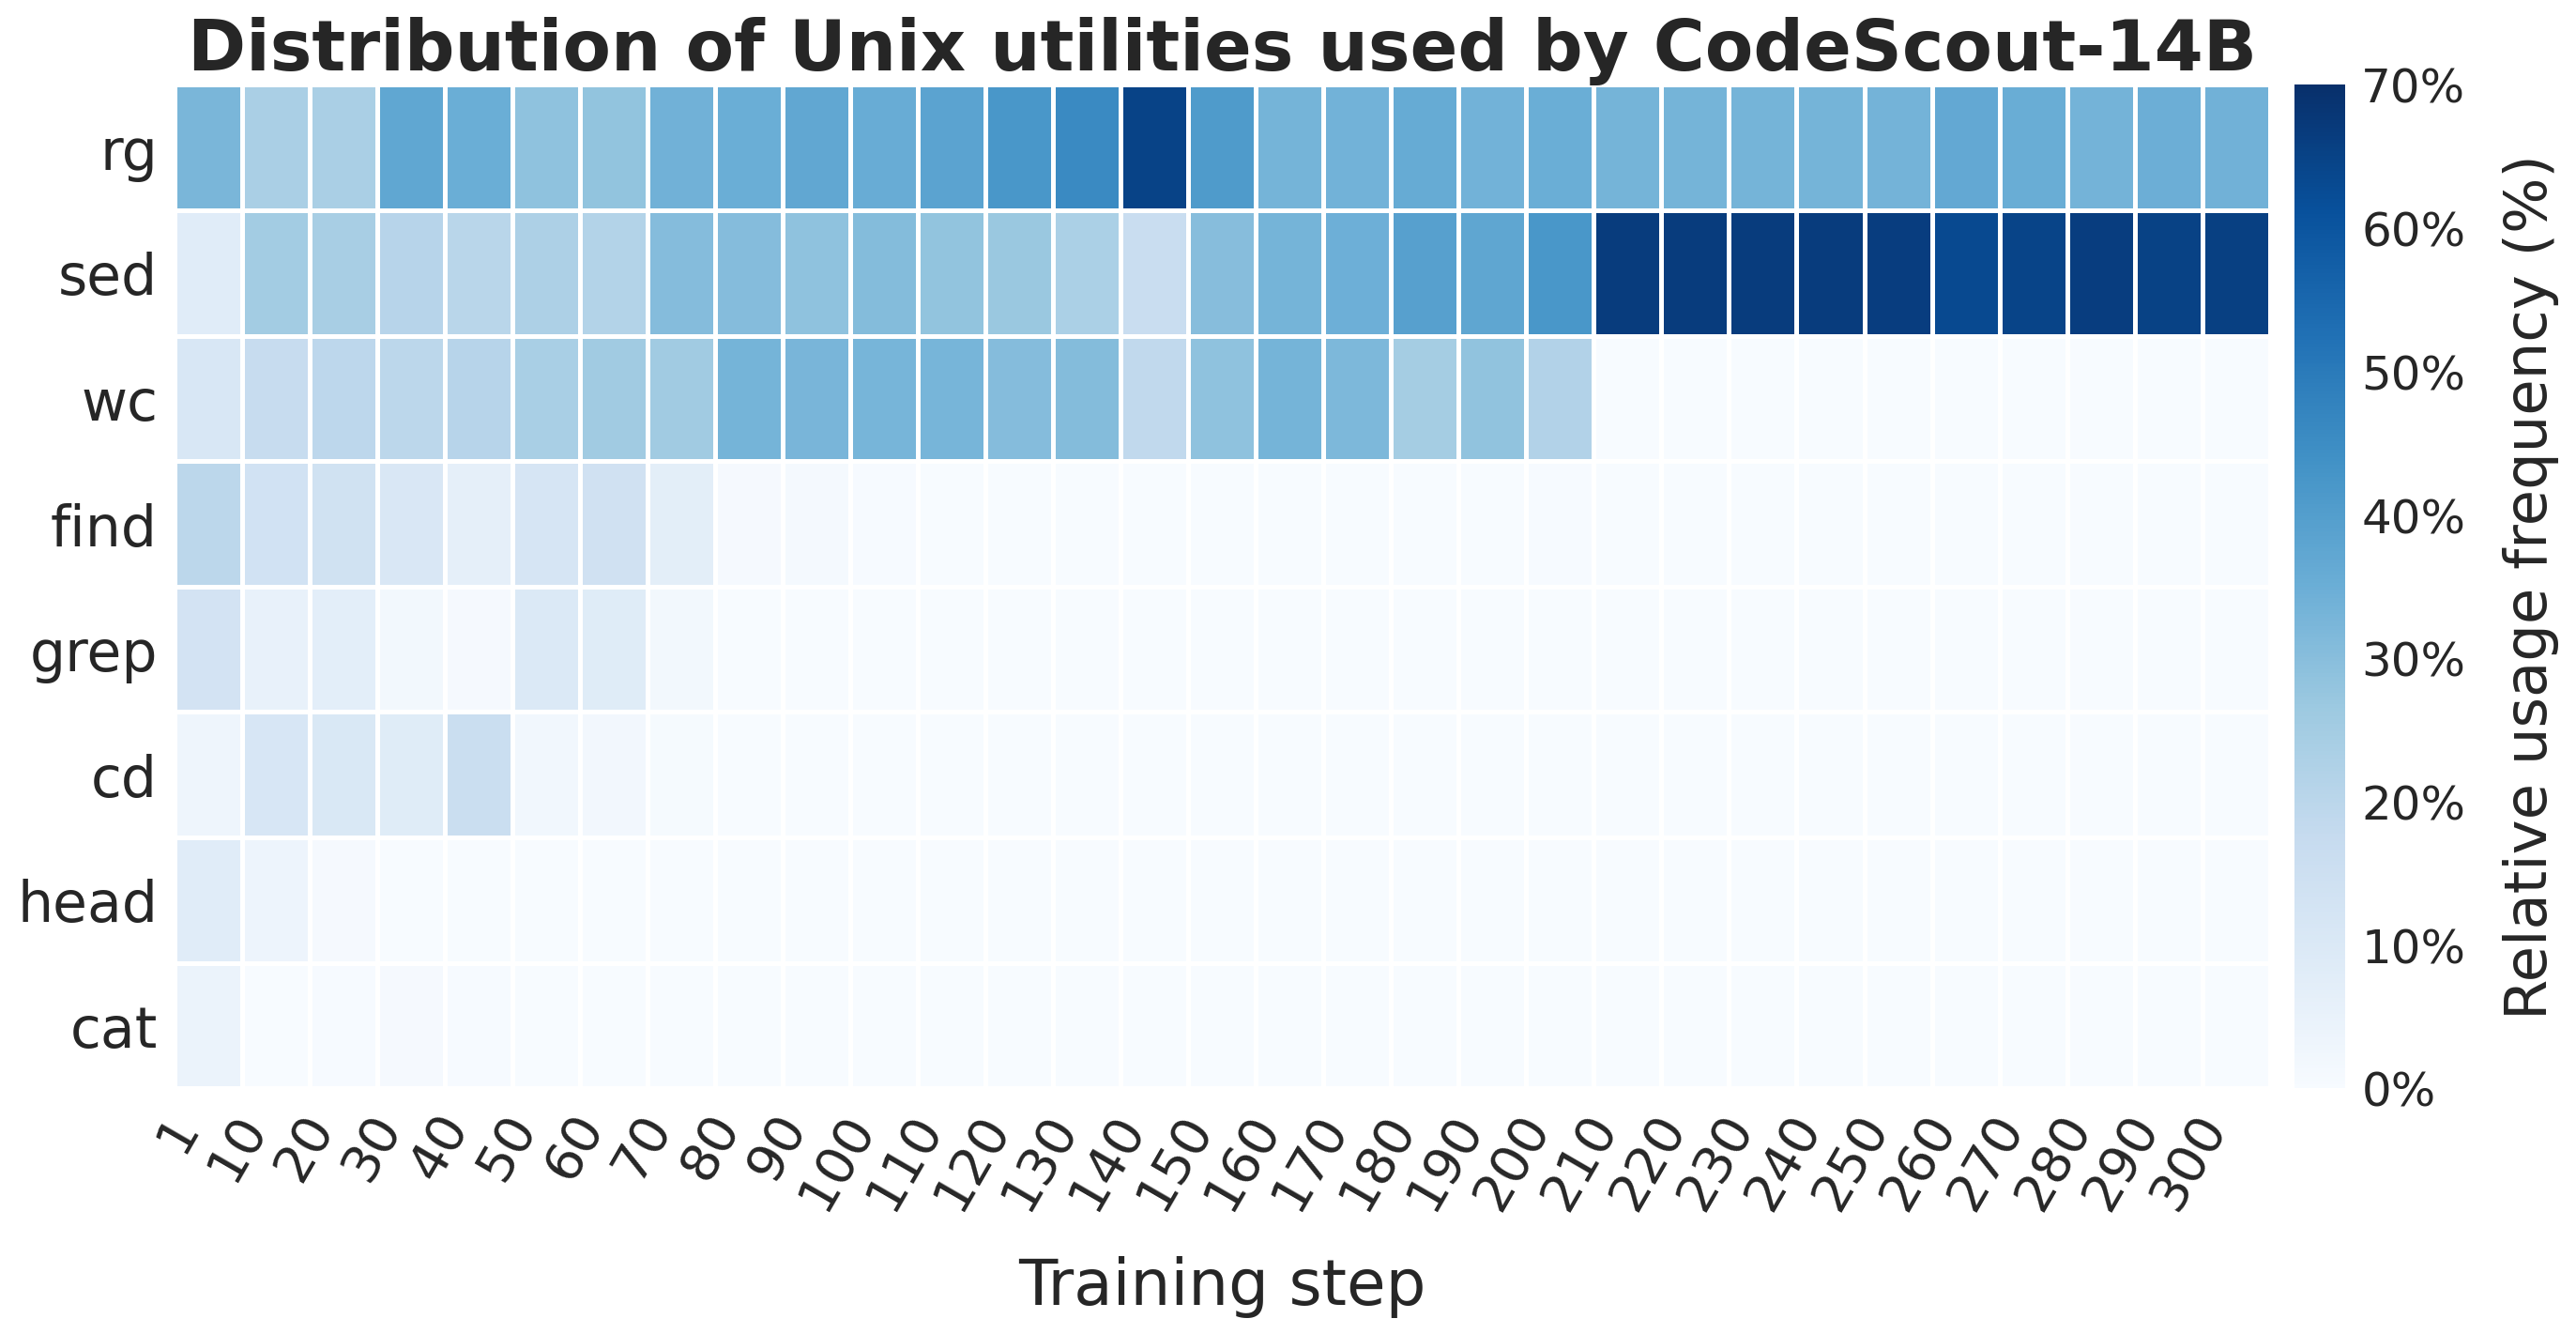
\includegraphics[width=\linewidth, height=\figheight]{Figures/command_relative_freq_14b.png}
        \caption{Tool use for \methodname-14B}
        \label{fig:tool_use_14b_sub}
    \end{subfigure}
    \hfill
    \begin{subfigure}[b]{\figwidth}
        \centering
        % Specifying both height and width forces the images to match exactly
        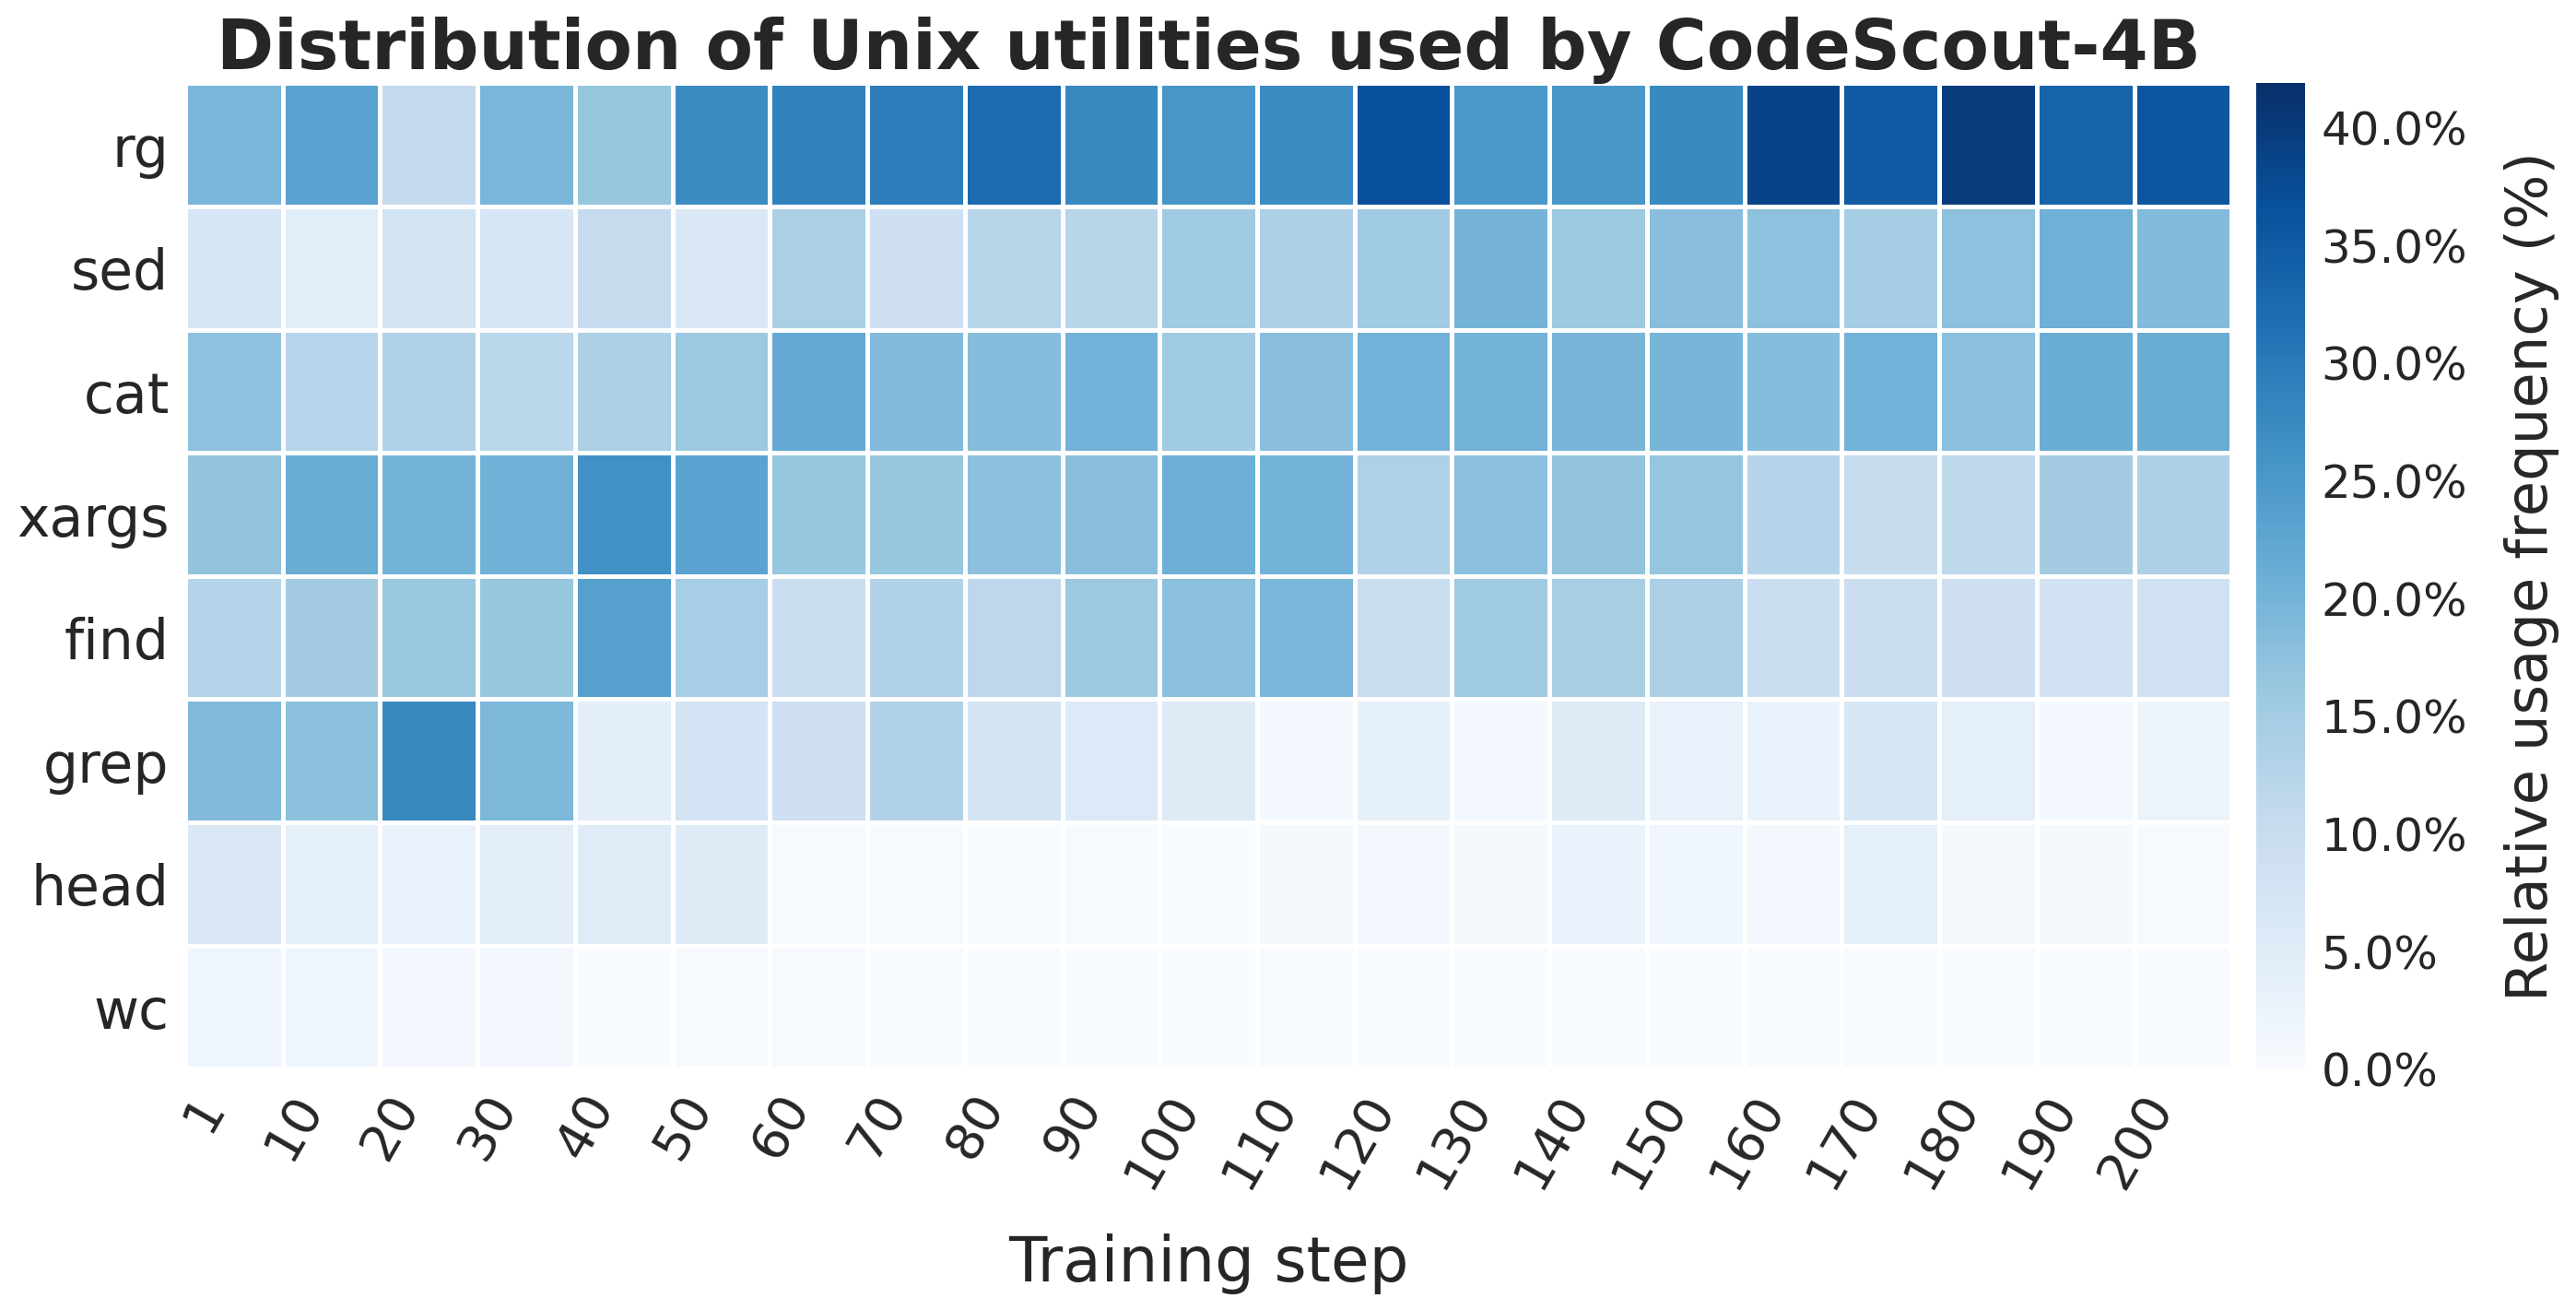
\includegraphics[width=\linewidth, height=\figheight]{Figures/command_relative_freq_4b.png}
        \caption{Tool use for \methodname-4B}
        \label{fig:tool_use_4b_sub}
    \end{subfigure}
    \caption{Distribution of the top-8 frequent commands used by \methodname. LLMs start with diverse utilities and converge to a small set as training proceeds. \methodname-14B uses only ripgrep (rg) and sed, while \methodname-4B mainly uses rg, cat, sed, and xargs.}
    \label{fig:merged_tool_use}
    \Description{Two subfigures showing a heatmap of the relative frequency of the top-8 most used Unix commands by CodeScout-14B and CodeScout-4B during training. The x-axis represents training steps and the y-axis lists the relative frequencies of each of top-8 commands.}
\end{figure*}

% \begin{figure}[h]
%     \centering
%     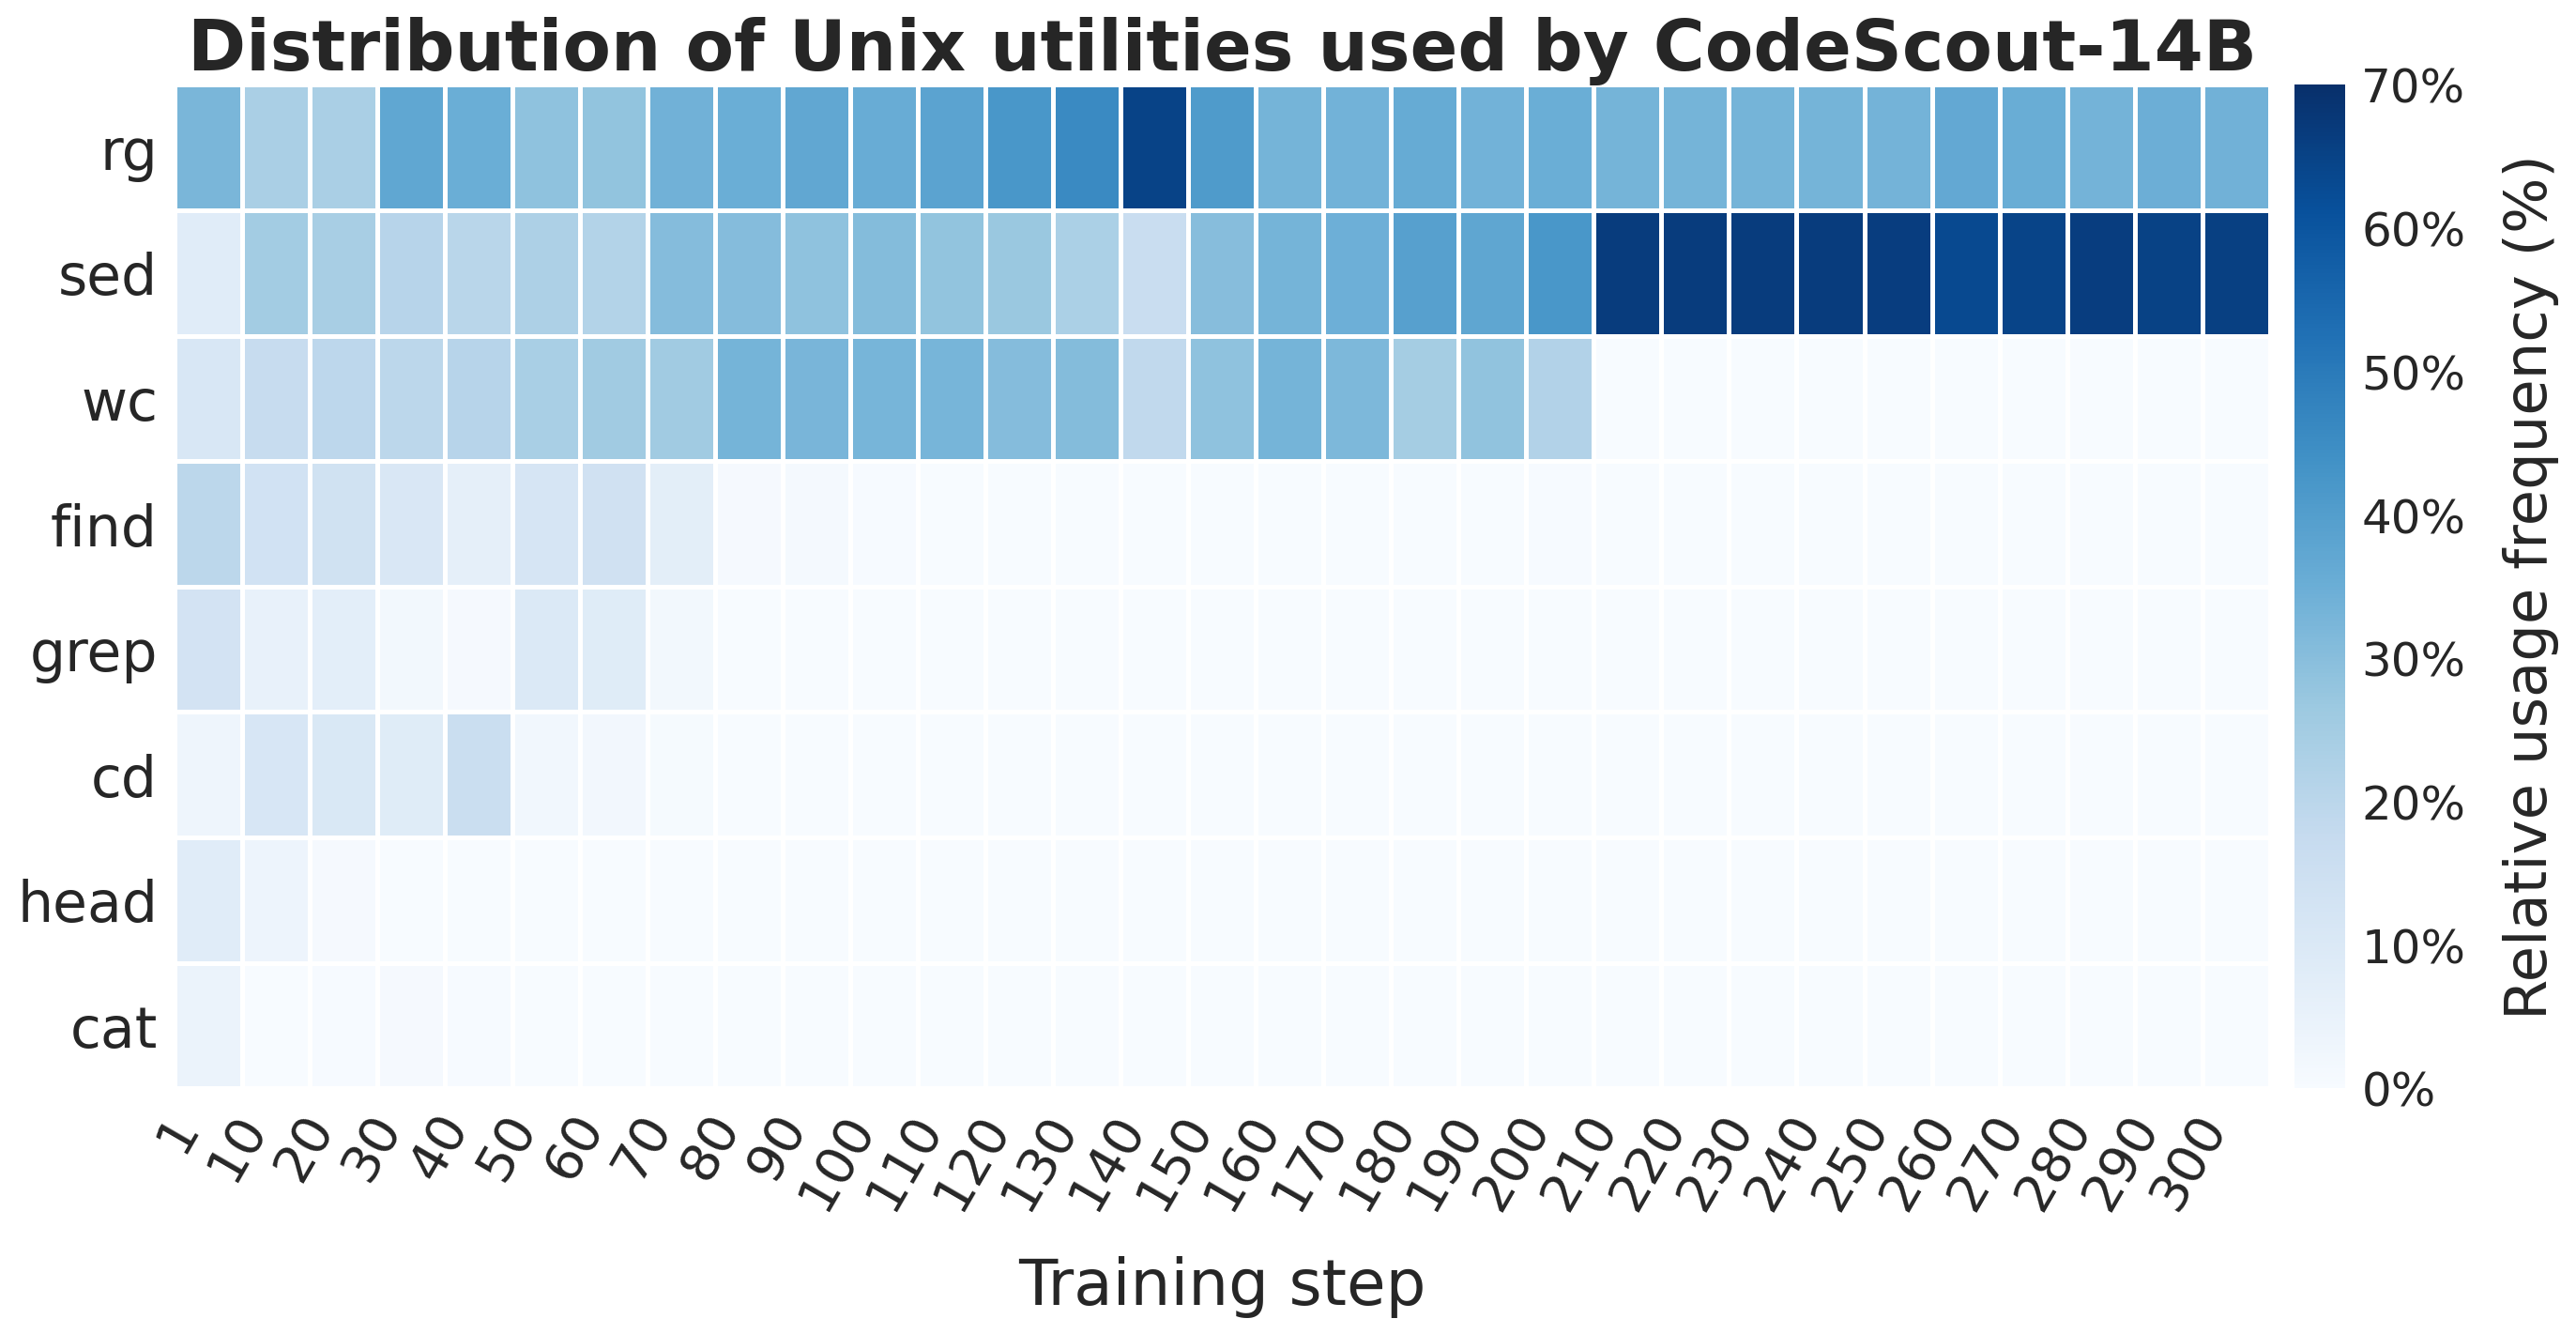
\includegraphics[width=\columnwidth]{Figures/command_relative_freq_14b.png}
%     \caption{Distribution of the top-8 most frequent Unix commands used by \methodname-14B measured using the relative usage frequency at different training steps during RL. \methodname-14B eventually converges to using just just two Unix commands, ripgrep and sed, and yet achieves strong code localization results.}
%     \label{fig:tool_use}
% \end{figure}

% \begin{table}[!t]
\centering
\caption{Issue resolution performance on SWE-Bench Verified: augmenting the agent with relevant locations improves performance and efficiency. Best metric is \textbf{bold-faced} and 2$^{nd}$ best is underlined.}
\renewcommand{\arraystretch}{1.1}
\setlength{\tabcolsep}{2.3pt}
\resizebox{\columnwidth}{!}{%
\begin{tabular}{lcccc} % Removed vertical bar for a cleaner look
\toprule
\makecell[l]{\textbf{Localization }\\\textbf{Approach}} & \makecell{\textbf{Resolution}\\\textbf{Rate $\uparrow$}} & \makecell{\textbf{Avg. \# }\\\textbf{Steps $\downarrow$}} & \makecell{\textbf{Avg. Input}\\\textbf{Tokens $\downarrow$}} & \makecell{\textbf{Avg. Output}\\\textbf{Tokens $\downarrow$}} \\
\midrule
\rowcolor{blue!15!white}\multicolumn{5}{c}{\textbf{Qwen3-4B-Instruct}} \\
\midrule
None (Vanilla) & 13.40\% & \underline{16.09} & 344.37K & \underline{2.98K} \\
\methodname-14B & \underline{17.20\%} & \textbf{13.91} & \textbf{284.26K} & \textbf{2.78K} \\
Oracle & \textbf{19.60\%} & 16.41 & \underline{327.75K} & 3.17K \\
\midrule
\rowcolor{pink!40!white}\multicolumn{5}{c}{\textbf{Qwen3-Coder-30B-A3B-Instruct}} \\ % Defined lightgolden color
\midrule
None (Vanilla) & 45.20\% & 51.00 & 1596.71K & 13.49K \\
\methodname-14B & \underline{46.00\%} & \underline{48.11} & \underline{1511.53K} & \underline{13.22K} \\
Oracle & \textbf{52.00\%} & \textbf{46.74} & \textbf{1358.60K} & \textbf{12.48K} \\
\bottomrule
\end{tabular}%
}
\label{tab:downstream_swe_bench}
\end{table}

    % \centering
    % % \vspace{-15pt} % Adjust vertical alignment as needed
    % \resizebox{0.5\columnwidth}{!}{%
    %     \renewcommand{\arraystretch}{1.1}
    %     \begin{tabular}{lcccc}
    %     \toprule
    %     \makecell[l]{\textbf{Localization }\\\textbf{Approach}} & \makecell{\textbf{Resolution}\\\textbf{Rate $\uparrow$}} & \makecell{\textbf{Avg. \# }\\\textbf{Steps $\downarrow$}} & \makecell{\textbf{Avg. Input}\\\textbf{Tokens $\downarrow$}} & \makecell{\textbf{Avg. Output}\\\textbf{Tokens $\downarrow$}} \\
    %     \midrule
    %     \rowcolor{blue!15!white}\multicolumn{5}{c}{\textbf{Qwen3-4B-Instruct}} \\
    %     \midrule
    %     None (Vanilla) & 13.40\% & \underline{16.09} & 344.37K & \underline{2.98K} \\
    %     \methodname-14B & \underline{17.20\%} & \textbf{13.91} & \textbf{284.26K} & \textbf{2.78K} \\
    %     Oracle & \textbf{19.60\%} & 16.41 & \underline{327.75K} & 3.17K \\
    %     \midrule
    %     \rowcolor{pink!40!white}\multicolumn{5}{c}{\textbf{Qwen3-Coder-30B-A3B-Instruct}} \\
    %     \midrule
    %     None (Vanilla) & 45.20\% & 51.00 & 1596.71K & 13.49K \\
    %     \methodname-14B & \underline{46.00\%} & \underline{48.11} & \underline{1511.53K} & \underline{13.22K} \\
    %     Oracle & \textbf{52.00\%} & \textbf{46.74} & \textbf{1358.60K} & \textbf{12.48K} \\
    %     \bottomrule
    %     \end{tabular}%
    % }
    % \label{tab:downstream_swe_bench}
% \begin{table}[!t]
% \caption{Issue resolution performance on SWE-Bench Verified: augmenting the agent with relevant code locations achieves higher resolution rate with fewer steps and token usage.}
% \centering
% \renewcommand{\arraystretch}{1.2}
% \setlength{\tabcolsep}{2.7pt}
% \resizebox{\columnwidth}{!}{%
% \begin{tabular}{ll|cccc}
% \toprule
% \textbf{LLM} & \makecell[l]{\textbf{Localization}\\\textbf{Approach}} & \makecell{\textbf{Resolution }\\\textbf{Rate $\uparrow$}} & \makecell{\textbf{Avg. }\\\textbf{\# Steps $\downarrow$}} & \makecell{\textbf{Avg. Input}\\\textbf{Tokens $\downarrow$}} & \makecell{\textbf{Avg. Output}\\\textbf{Tokens $\downarrow$}} \\
% \midrule
% \multirow{3}{*}{\textbf{\makecell[l]{Qwen3-4B-\\Instr.}}} & None (Vanilla) & 13.40\% & \underline{16.09} & 344.37K & \underline{2.98K} \\
% & \methodname-14B & \underline{17.20\%} & \textbf{13.91} & \textbf{284.26K} & \textbf{2.78K} \\
% & Oracle & \textbf{19.60\%} & 16.41 & \underline{327.75K} & 3.17K \\
% \midrule
% \multirow{3}{*}{\textbf{\makecell[l]{Qwen3-Coder-\\30B-A3B-Instr.}}} & None (Vanilla) & 45.20\% & 51.00 & 1596.71K & 13.49K \\
% & \methodname-14B & \underline{46.00\%} & \underline{48.11} & \underline{1511.53K} & \underline{13.22K} \\
% & Oracle & \textbf{52.00\%} & \textbf{46.74} & \textbf{1358.60K} & \textbf{12.48K} \\
% \bottomrule
% \end{tabular}%
% }
% \label{tab:downstream_swe_bench}
% \end{table}
% if two-column table preferred see below
% \begin{table*}[h]
% \caption{Downstream performance on \textbf{SWE-Bench Verified} using different localization methods. \methodname localization consistently improves issue resolution rates and reduces the average number of steps and token consumption compared to the vanilla baseline.}
% \centering
% \renewcommand{\arraystretch}{1.2}
% \setlength{\tabcolsep}{6.0pt}
% \resizebox{\textwidth}{!}{%
% \begin{tabular}{ll|cccc}
% \toprule
% \textbf{LLM} & \textbf{Localization Approach} & \textbf{Resolution Rate $\uparrow$} & \textbf{Avg. \# Steps $\downarrow$} & \textbf{Avg. Input Tokens $\downarrow$} & \textbf{Avg. Output Tokens $\downarrow$} \\
% \midrule
% \multirow{3}{*}{\textbf{Qwen3-4B-Instruct-2507}} & None (Vanilla Setup) & 13.40\% & \underline{16.09} & 344.37K & \underline{2.98K} \\
% & \methodname-14B & \underline{17.20\%} & \textbf{13.91} & \textbf{284.26K} & \textbf{2.78K} \\
% & Oracle (using gold patch) & \textbf{19.60\%} & 16.41 & \underline{327.75K} & 3.17K \\
% \midrule
% \multirow{3}{*}{\textbf{Qwen3-Coder-30B-A3B-Instruct}} & None (Vanilla Setup) & 45.20\% & 51.00 & 1596.71K & 13.49K \\
%  & \methodname-14B & \underline{46.00\%} & \underline{48.11} & \underline{1511.53K} & \underline{13.22K} \\
% & Oracle (using gold patch) & \textbf{52.00\%} & \textbf{46.74} & \textbf{1358.60K} & \textbf{12.48K} \\
% \bottomrule
% \end{tabular}%
% }
% \label{tab:downstream_swe_bench}
% \end{table*}
We show that augmenting OpenHands issue resolution agent~\citep{wang2025openhandssoftwareagentsdk} with relevant code retrieved by \methodname improves performance on SWE-Bench Verified. We consider three settings: (1) a vanilla baseline without localization, (2) augmenting the agent with locations retrieved by \methodname-14B, and (3) augmenting the agent with oracle locations parsed from the gold patch (\S\ref{sec:data_creation}). 
For (2) and (3), the user prompt is modified to include the names of localized files, modules, and functions (Appendix~\ref{appendix:prompts_swe_bench}). We evaluate Qwen3-4B-Instruct-2507 and Qwen3-Coder-30B-A3B-Instruct compare the performance of the three settings using issue resolution rate, and their efficiency using instance-level averages of the number of steps per trajectory and the total input and output tokens accumulated across all turns. Table~\ref{tab:downstream_swe_bench} presents the detailed results.
% \begin{wraptable}{r}{0.5\columnwidth}
% \end{wraptable}
\begin{table}[!t]
\centering
\caption{Issue resolution performance on SWE-Bench Verified: augmenting the agent with relevant locations improves performance and efficiency. Best metric is \textbf{bold-faced} and 2$^{nd}$ best is underlined.}
\renewcommand{\arraystretch}{1.1}
\setlength{\tabcolsep}{2.3pt}
\resizebox{\columnwidth}{!}{%
\begin{tabular}{lcccc} % Removed vertical bar for a cleaner look
\toprule
\makecell[l]{\textbf{Localization }\\\textbf{Approach}} & \makecell{\textbf{Resolution}\\\textbf{Rate $\uparrow$}} & \makecell{\textbf{Avg. \# }\\\textbf{Steps $\downarrow$}} & \makecell{\textbf{Avg. Input}\\\textbf{Tokens $\downarrow$}} & \makecell{\textbf{Avg. Output}\\\textbf{Tokens $\downarrow$}} \\
\midrule
\rowcolor{blue!15!white}\multicolumn{5}{c}{\textbf{Qwen3-4B-Instruct}} \\
\midrule
None (Vanilla) & 13.40\% & \underline{16.09} & 344.37K & \underline{2.98K} \\
\methodname-14B & \underline{17.20\%} & \textbf{13.91} & \textbf{284.26K} & \textbf{2.78K} \\
Oracle & \textbf{19.60\%} & 16.41 & \underline{327.75K} & 3.17K \\
\midrule
\rowcolor{pink!40!white}\multicolumn{5}{c}{\textbf{Qwen3-Coder-30B-A3B-Instruct}} \\ % Defined lightgolden color
\midrule
None (Vanilla) & 45.20\% & 51.00 & 1596.71K & 13.49K \\
\methodname-14B & \underline{46.00\%} & \underline{48.11} & \underline{1511.53K} & \underline{13.22K} \\
Oracle & \textbf{52.00\%} & \textbf{46.74} & \textbf{1358.60K} & \textbf{12.48K} \\
\bottomrule
\end{tabular}%
}
\label{tab:downstream_swe_bench}
\end{table}

    % \centering
    % % \vspace{-15pt} % Adjust vertical alignment as needed
    % \resizebox{0.5\columnwidth}{!}{%
    %     \renewcommand{\arraystretch}{1.1}
    %     \begin{tabular}{lcccc}
    %     \toprule
    %     \makecell[l]{\textbf{Localization }\\\textbf{Approach}} & \makecell{\textbf{Resolution}\\\textbf{Rate $\uparrow$}} & \makecell{\textbf{Avg. \# }\\\textbf{Steps $\downarrow$}} & \makecell{\textbf{Avg. Input}\\\textbf{Tokens $\downarrow$}} & \makecell{\textbf{Avg. Output}\\\textbf{Tokens $\downarrow$}} \\
    %     \midrule
    %     \rowcolor{blue!15!white}\multicolumn{5}{c}{\textbf{Qwen3-4B-Instruct}} \\
    %     \midrule
    %     None (Vanilla) & 13.40\% & \underline{16.09} & 344.37K & \underline{2.98K} \\
    %     \methodname-14B & \underline{17.20\%} & \textbf{13.91} & \textbf{284.26K} & \textbf{2.78K} \\
    %     Oracle & \textbf{19.60\%} & 16.41 & \underline{327.75K} & 3.17K \\
    %     \midrule
    %     \rowcolor{pink!40!white}\multicolumn{5}{c}{\textbf{Qwen3-Coder-30B-A3B-Instruct}} \\
    %     \midrule
    %     None (Vanilla) & 45.20\% & 51.00 & 1596.71K & 13.49K \\
    %     \methodname-14B & \underline{46.00\%} & \underline{48.11} & \underline{1511.53K} & \underline{13.22K} \\
    %     Oracle & \textbf{52.00\%} & \textbf{46.74} & \textbf{1358.60K} & \textbf{12.48K} \\
    %     \bottomrule
    %     \end{tabular}%
    % }
    % \label{tab:downstream_swe_bench}
% \begin{table}[!t]
% \caption{Issue resolution performance on SWE-Bench Verified: augmenting the agent with relevant code locations achieves higher resolution rate with fewer steps and token usage.}
% \centering
% \renewcommand{\arraystretch}{1.2}
% \setlength{\tabcolsep}{2.7pt}
% \resizebox{\columnwidth}{!}{%
% \begin{tabular}{ll|cccc}
% \toprule
% \textbf{LLM} & \makecell[l]{\textbf{Localization}\\\textbf{Approach}} & \makecell{\textbf{Resolution }\\\textbf{Rate $\uparrow$}} & \makecell{\textbf{Avg. }\\\textbf{\# Steps $\downarrow$}} & \makecell{\textbf{Avg. Input}\\\textbf{Tokens $\downarrow$}} & \makecell{\textbf{Avg. Output}\\\textbf{Tokens $\downarrow$}} \\
% \midrule
% \multirow{3}{*}{\textbf{\makecell[l]{Qwen3-4B-\\Instr.}}} & None (Vanilla) & 13.40\% & \underline{16.09} & 344.37K & \underline{2.98K} \\
% & \methodname-14B & \underline{17.20\%} & \textbf{13.91} & \textbf{284.26K} & \textbf{2.78K} \\
% & Oracle & \textbf{19.60\%} & 16.41 & \underline{327.75K} & 3.17K \\
% \midrule
% \multirow{3}{*}{\textbf{\makecell[l]{Qwen3-Coder-\\30B-A3B-Instr.}}} & None (Vanilla) & 45.20\% & 51.00 & 1596.71K & 13.49K \\
% & \methodname-14B & \underline{46.00\%} & \underline{48.11} & \underline{1511.53K} & \underline{13.22K} \\
% & Oracle & \textbf{52.00\%} & \textbf{46.74} & \textbf{1358.60K} & \textbf{12.48K} \\
% \bottomrule
% \end{tabular}%
% }
% \label{tab:downstream_swe_bench}
% \end{table}
% if two-column table preferred see below
% \begin{table*}[h]
% \caption{Downstream performance on \textbf{SWE-Bench Verified} using different localization methods. \methodname localization consistently improves issue resolution rates and reduces the average number of steps and token consumption compared to the vanilla baseline.}
% \centering
% \renewcommand{\arraystretch}{1.2}
% \setlength{\tabcolsep}{6.0pt}
% \resizebox{\textwidth}{!}{%
% \begin{tabular}{ll|cccc}
% \toprule
% \textbf{LLM} & \textbf{Localization Approach} & \textbf{Resolution Rate $\uparrow$} & \textbf{Avg. \# Steps $\downarrow$} & \textbf{Avg. Input Tokens $\downarrow$} & \textbf{Avg. Output Tokens $\downarrow$} \\
% \midrule
% \multirow{3}{*}{\textbf{Qwen3-4B-Instruct-2507}} & None (Vanilla Setup) & 13.40\% & \underline{16.09} & 344.37K & \underline{2.98K} \\
% & \methodname-14B & \underline{17.20\%} & \textbf{13.91} & \textbf{284.26K} & \textbf{2.78K} \\
% & Oracle (using gold patch) & \textbf{19.60\%} & 16.41 & \underline{327.75K} & 3.17K \\
% \midrule
% \multirow{3}{*}{\textbf{Qwen3-Coder-30B-A3B-Instruct}} & None (Vanilla Setup) & 45.20\% & 51.00 & 1596.71K & 13.49K \\
%  & \methodname-14B & \underline{46.00\%} & \underline{48.11} & \underline{1511.53K} & \underline{13.22K} \\
% & Oracle (using gold patch) & \textbf{52.00\%} & \textbf{46.74} & \textbf{1358.60K} & \textbf{12.48K} \\
% \bottomrule
% \end{tabular}%
% }
% \label{tab:downstream_swe_bench}
% \end{table*}
For Qwen3-4B-Instruct, augmenting the agent with locations retrieved by \methodname-14B increases the resolution rate by \textbf{3.8\%}, while reducing trajectory length by \textbf{2.18} steps, and input and output tokens by \textbf{17.46\%} and \textbf{6.71\%} respectively. Similar efficiency gains are observed for Qwen3-Coder-30B-A3B-Instruct, with \textbf{2.89} fewer steps and \textbf{5.33\%} fewer input tokens and \textbf{2.00\%} fewer output tokens, while achieving comparable performance with a small improvement (+0.80\%). For both LLMs, replacing \methodname predictions with oracle locations yields further performance gains (\textbf{+6.00\%} for 30B and \textbf{+2.40\%} for 4B). The 30B model also benefits with improved efficiency, with \textbf{1.37} fewer steps and reductions of \textbf{10.12\%} and \textbf{5.60\%} in input and output tokens. Overall, these results indicate that continued improvements in code localization will further enhance both the performance and efficiency of issue resolution agents.

\subsection{How does the tool-use behaviour of \methodname evolve during RL?}\label{sec:tool_use_behaviour}
To analyze the evolving tool-use behaviors RL, we plot the distribution of Unix utilities invoked by the LLM in Figure~\ref{fig:merged_tool_use}. We parse rollouts sampled from model checkpoints at every 10 training steps and aggregate command usage across these checkpoints to identify the top-8 frequently used commands. For each checkpoint, we compute the relative usage frequency of each utility for all rollouts logged in that training step.

We observe convergence in tool usage during RL. While the 14B LLM initially uses various utilities, after 200 training steps it uses \emph{only} on two commands: \texttt{ripgrep} (\texttt{rg}) and \texttt{sed}. Similarly, while the 4B LLM initially uses many utilities, it converges to mainly using \texttt{ripgrep}, \texttt{sed}, \texttt{cat}, \texttt{find} and \texttt{xargs}. Thus, we can further simplify the agent to a small subset of Unix utilities without needing access to the entire terminal which is crucial in security-sensitive deployments. Appendix~\ref{appendix:traj_examples} presents example trajectories for 4B and 14B LLMs that illustrate how these utilities are used by the agent.
% We provided analysis of evolving tool-use behaviours of \methodname-4B and \methodname-14B during their respective RL training runs. For all training steps, we parse the Unix utilities from the raw commands issued by the agent when using the \texttt{Terminal} tool across all turns in each sampled rollout. We restrict our analysis to the top-8 Unix utilities based on their total usage frequency across over the entire training run. Finally, we plot the heatmap of the relative usage frequencies of these utilities for every 10 training steps, 

% In Figure \ref{fig:merged_tool_use}, we observe that at the start of training, \methodname tries out multiple different bash commands such as \texttt{cat}, \texttt{grep}, etc. However, as training progresses, the agent quickly converges to using less command variations and after 250 steps only uses \texttt{rg} and \texttt{sed}. This is most likely due to the \texttt{rg} command being comprehensive enough as functionalities from \texttt{cat}, \texttt{find}, and \texttt{grep} can be done with \texttt{rg}. \texttt{cd} also sees dimishing use likely due to the the more effective use of \texttt{rg} that makes changing directory unnecessary.